\begin{frame}{Paper Review}
    ``Consensus-Based Decentralized Auctions for Robust Task Allocation" by  Choi et al. \cite{choi2009consensus}
    \begin{itemize}
        \item Assignment Algorithm
        \item Guarantees
        \item Numerical Results
        \item Strengths and Weaknesses 
    \end{itemize}
\end{frame}

% \begin{frame}{Paper Review - CBAA}
%     \begin{columns}
%     \begin{column}{0.65\textwidth}
%     \begin{itemize}
%         \item CBAA is for the single linear assignment problem in Eq.~\eqref{linear_assign} consisting of auction and consensus phases
%         \pause
%         \item Auction phase: 
%         \begin{itemize}
%             \item Each robot has a local winning bid list $\mathbf{y}_i \in \reals_{+}^{N_t}$
%             \item Independently choose an unassigned task with the largest $c_{ij} \in \reals_{+}$ and $c_{ij} > y_{ij}$ (denote this task $J_i$)
%             \item Update component $y_{i,J_i} = c_{i,J_i}$
%         \end{itemize} 
%         \pause
%         \item Consensus phase: 
%         \begin{itemize}
%             \item Communicate winning bid list $\mathbf{y}_i$ with neighbors 
%             \item Do maximum consensus on the components of $\mathbf{y}_i$
%             \item Loose task assignment if another robot has a higher bid
%         \end{itemize} 
%     \end{itemize}
%     \end{column}
%     \begin{column}{0.5\textwidth}
%     \onslide<1->
%     \begin{equation}
%             \label{linear_assign}
%             \begin{aligned}
%             & \max \quad \sum_{i=1}^{N_u} \sum_{j=1}^{N_t} {\color{red}c_{ij}} \cdot x_{ij} \\
%             % &  \\
%             & \text{s.t} \quad \sum_{j=1}^{N_t} x_{ij} \leq {\color{red}L_t = 1} \quad \forall i \in \mathcal{I}, \\
%             & \sum_{i=1}^{N_u} x_{ij} \leq 1 \quad \forall j \in \mathcal{J}, \\
%             & \sum_{i=1}^{N_u} \sum_{j=1}^{N_t} x_{ij} = \min \{N_t, N_u\},  \\ 
%             & x_{ij} \in \{0, 1\} \quad \forall (i,j) \in \mathcal{I} \times \mathcal{J}.
%             \end{aligned}
%     \end{equation}
%     \end{column}
%     \end{columns}
% \end{frame}

\begin{frame}{Paper Review - CBBA}
    \begin{itemize}
        \item Introduces Consensus-Based Auction Algorithm (CBAA) for the linear single-assignment 
       \begin{figure}
            \centering
            {
            \includegraphics[width=0.4\linewidth]{Figures/CBAA.pdf}}
            % \caption{CBAA for single assignment (left), CBBA for multi assignment (right) }
        \end{figure}
        \pause
        \item Generalize to Consensus-Based Bundle Algorithm (CBBA) to assign a sequence of tasks in a path vector
        % \begin{itemize}
        %     \item Assignments are done on the task level, not the bundle level
        % \end{itemize}
        \visible<2>{
        \begin{figure}
            \centering
            {
            \includegraphics[width=0.62\linewidth]{Figures/CBBA.pdf}}
            % \caption{CBAA for single assignment (left), CBBA for multi assignment (right) }
        \end{figure}}
        
        % \item Scoring function depends on the path vector, i.e., $c_{ij}(\mathbf{p}_i)$ 
        % \item CBBA does the TA on the task level, not the vector level
        % \item Each robot has,
        % \begin{itemize}
        %     \item Bundle $\mathbf{b}_i \in (\mathcal{J} \cup \{\emptyset\})^{L_t}$: a list of tasks ordered based on which task was added first
        %     \item Path vector $\mathbf{p}_i \in (\mathcal{J} \cup \{\emptyset\})^{L_t}$: a list of tasks ordered based on their location in the assignment
        % \end{itemize}
    \end{itemize}
\end{frame}

\begin{frame}{Paper Review - CBBA}
    \begin{itemize}
        \item CBBA consists of bundle construction and consensus iterations
        \item Bundle construction (at each iteration):
        \begin{itemize}
            \item Bundle $\mathbf{b}_i$: a list of tasks ordered based on which task was \textbf{added first}
            \item Path vector $\mathbf{p}_i$: a list of tasks ordered based on their \textbf{location in the assignment}
        \end{itemize}
        \visible<2>{
          \begin{figure}
            \centering
            {
            \includegraphics[width=0.9\linewidth]{Figures/bundle_construction_1.pdf}}
        \end{figure}
        }
    \end{itemize}
\end{frame}

\begin{frame}{Paper Review - CBBA}
    \begin{itemize}
        \item CBBA consists of bundle construction and consensus iterations
        \item Bundle construction (at each iteration):
        \begin{itemize}
            \item Bundle $\mathbf{b}_i$: a list of tasks ordered based on which task was \textbf{added first}
            \item Path vector $\mathbf{p}_i$: a list of tasks ordered based on their \textbf{location in the assignment}
        \end{itemize}
          \begin{figure}
            \centering
            {
            \includegraphics[width=0.9\linewidth]{Figures/bundle_construction_2.pdf}}
        \end{figure}
    \end{itemize}
\end{frame}

\begin{frame}{Paper Review - CBBA}
    \begin{itemize}
        \item Robot $i$ adds unassigned tasks to its bundle and path vector greedily, with the largest marginal score improvement
        \begin{equation*}
            c_{ik}[\mathbf{b}_i] = \max_{n:n\le |\mathbf{p}_i|}\left( \underbrace{S_{i}^{\mathbf{p}_i \oplus_n \{k\}}}_{\text{reward from path $\mathbf{p}_i \oplus_n \{k\}$}} - \underbrace{S_{i}^{\mathbf{p}_i}}_{\text{reward from path $\mathbf{p}_i$}} \right),
        \end{equation*}
        where the best task among all tasks is 
            $k^* = \argmax_{k} \left(c_{ik}[\mathbf{b}_i]\right)$.
        \visible<2>{
        \begin{figure}
            \centering
            {
            \includegraphics[width=0.85\linewidth]{Figures/bundle_construction_3.pdf}}
        \end{figure}
        }
    \end{itemize}
\end{frame}

\begin{frame}{Paper Review - CBBA}
    \begin{itemize}
        \item Keep adding tasks to the bundle and path vector until they are filled
        \item Robot $i$ also associates each chosen task with itself (for consensus)
        \begin{itemize}
            \item $\mathbf{y}_i$: winning bid list
            \item $\mathbf{z}_i$: winning robot list
        \end{itemize}
        \begin{figure}
            \centering
            {
            \includegraphics[width=0.95\linewidth]{Figures/bundle_construction_4.pdf}}
        \end{figure}
    \end{itemize}
\end{frame}

\begin{frame}{Paper Review - CBBA}
    \begin{itemize}
        \item Consensus phase for resolving any conflicting task assignments
        \begin{itemize}
            \item Robots communicate
            \begin{itemize}
                \item $\mathbf{y}_i$: winning bid list
                \item $\mathbf{z}_i$: winning robot list
                \item $\mathbf{s}_i$:  time stamp vector for the last information update from other robots
            \end{itemize}
            \pause
            \item Each robot either updates, resets, or keeps its assignment based on $\mathbf{y}_i, \mathbf{z}_i, \mathbf{s}_i$ and decision rules, which are roughly maximum consensus 
        \end{itemize}
        \visible<2>{
        \begin{figure}
            \centering
            {
            \includegraphics[width=0.95\linewidth]{Figures/consensus_network.pdf}}
        \end{figure}
        }
    \end{itemize}

\end{frame}

\begin{frame}{Paper Review - CBBA Guarantees}
    \begin{itemize}
        \item Two main theorems, convergence and optimally of CBBA, under the following assumption
    \end{itemize}
    \begin{assum}[Diminishing Marginal Gain (DMG) on Scoring Function]
        The value of a task doesn't increase as other elements are added to the set before it, i.e., $$\underbrace{c_{ij}[\mathbf{b}_i]}_{\tiny \text{marginal improvement to } \mathbf{b}_i} \ge \underbrace{c_{ij}[\mathbf{b}_i \oplus_{\text{end}} \mathbf{b}]}_{\tiny \text{marginal improvement to } \mathbf{b}_i \oplus_{\text{end}} \mathbf{b}}$$
    \end{assum}
    \begin{itemize}
        \item The proof of the 2 theorems relies on a reduction of CBBA to a centralized sequential greedy algorithm (SGA).
    \end{itemize}
\end{frame}

\begin{frame}{Paper Review - CBBA Guarantees}
    \begin{theorem}[Convergence of CBBA]
        Provided DMG scoring functions and synchronized consensus over a static communication network
        \begin{columns}
        \begin{column}{0.56\textwidth}
        \begin{enumerate}
            \item CBBA produces the same solution as the sequential greedy algorithm (SGA)
            \item Convergence time is bounded above by $N_{\text{min}} \cdot D = \min \{N_t, N_u\cdot L_t\} \cdot D$ with network diameter $D$
        \end{enumerate}
        \end{column}
        \begin{column}{0.35\textwidth}
        \begin{figure}
            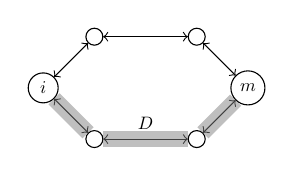
\begin{tikzpicture}[scale=0.65, transform shape]
            % Define the nodes
            \node[draw, circle] (i) at (1,0) {$i$};
            \node[draw, circle] (a) at (2,1) {};
            \node[draw, circle] (b) at (2,-1) {};
            \node[draw, circle] (c) at (4,1) {};
            \node[draw, circle] (d) at (4,-1) {};
            % \node[draw, circle] (e) at (3,1) {}; % New node
            \node[draw, circle] (j) at (5,0) {$m$};
        
            % Draw the edges
            \draw[<->] (i) -- (a);
            \draw[<->] (i) -- (b);
            % \draw (a) -- (c);
            \draw[<->] (b) -- (d);
            \draw[<->] (c) -- (j);
            \draw[<->] (d) -- (j);
            % \draw[<->] (a) -- (e);
            % \draw[<->] (c) -- (e);
            \draw[<->] (a) -- (c);
            % \draw[<->] (c) -- (e);
        
            % Highlight the diameter path
            \draw[line width=2mm, gray, opacity=0.5] (i) -- (b) -- (d) -- (j);
        
            % Add labels
            \node at (3,-0.7) {$D$};
            \end{tikzpicture}
            \caption{Diameter $D$}
        \end{figure}
        \end{column}
    \end{columns}
    \end{theorem}
    \begin{theorem}[Optimality of CBBA]
        Provided DMG scoring functions and accurate situational awareness, CBBA guarantees 50\% optimality for the MRTA.
    \end{theorem}
\end{frame}

\begin{frame}{Paper Review - Numerical Results}
    \begin{itemize}
        \item CBBA is analyzed under inconsistent situational awareness (SA), i.e., position estimates of the tasks among the robots
        \begin{itemize}
            \item Each robot has different estimates of the task positions
        \end{itemize}
    \end{itemize}
    \begin{figure}
        \centering
        \onslide<1->
        \subfloat[Convergence with inconsistent SA]{\includegraphics[width=0.45\linewidth]{Figures/convergence_time.png}}
        \hfill
        \subfloat[Optimality gap with inconsistent SA]{\includegraphics[width=0.45\linewidth]{Figures/optimality_gap.png}}
    \label{fig:2}
    \end{figure}
\end{frame}

\begin{frame}{Paper Review - Strengths and Weaknesses}
    \begin{block}{~\vspace{0.7cm}}
        \begin{center}
        \vspace{-1.0cm}
        \setcellgapes{4pt}\makegapedcells
        \begin{tabular}{>{\centering}p{0.45\textwidth}|>{\centering\arraybackslash}p{0.45\textwidth}}
         \textcolor{white}{\bfseries\boldmath Strengths} & \textcolor{white}{\bfseries Weaknesses} \\
        Computationally efficient %(no need for local copies of the problem)
        &  Assumes local information, i.e., SA relating to score functions, can be sensed/estimated by every robot \\ 
       Guaranteed conflict-free task assignments (even with inconsistent SA) & Score functions need to satisfy the diminishing marginal return property \\  
       Guaranteed to be at least 50\% optimal (although requires consistent SA)
        & 50\% optimal for CBAA (linear assignment case) \\ &  Requires synchronized consensus \\
        & No experiments
        \end{tabular}
        \end{center}
    \end{block}
\end{frame}
